\documentclass[11pt, a4paper]{article}

\usepackage[utf8]{inputenc}
\usepackage[top=2.5cm, left=1.5cm, text={18cm, 25cm}]{geometry}
\usepackage[IL2]{fontenc}
\usepackage{amsmath}
\usepackage{amsthm}
\usepackage{caption}
\usepackage[unicode]{hyperref}
\usepackage{graphicx}

\hypersetup{
    colorlinks=true,
    linkcolor=blue,
    filecolor=magenta,
    urlcolor=cyan,
}

\renewcommand{\figurename}{Button Image}
\title{proj2}
\author{Intr-net}
\date{March 2021}
\begin{document}
    \begin{titlepage}
        \begin{center}
            \vspace*{1cm}

            \huge
            \Huge F\huge AKULTA INFORMAČNÍCH TECHNOLOIÍ\\
            \hspace{0.2cm}
            \Huge V\huge YSOKÉ UČENÍ TECHNIOCKÉ V \Huge B\huge RNĚ\\
            \vspace{\stretch{0.382}}
            CALCULATOR \\
            MANUAL
            \vspace{\stretch{0.618}}


        \end{center}
        {\LARGE 2021 \hfill
        Intr-net}
    \end{titlepage}

    \newpage

    \tableofcontents


    \section{Usage}
    \t Usage of buttons with mathematical and logical functions.
    For more detailed description, open refman.pdf.
    \label{sec:usage}

    \subsection{Introduction}
    \label{subsec:Introduction}
    Our calculator app is split to parts. Buttons with: numbers, math operations, memory operations and display.
    Usage is simple and is described in subsection of each operation.
    \newline
    \begin{figure}[h]
        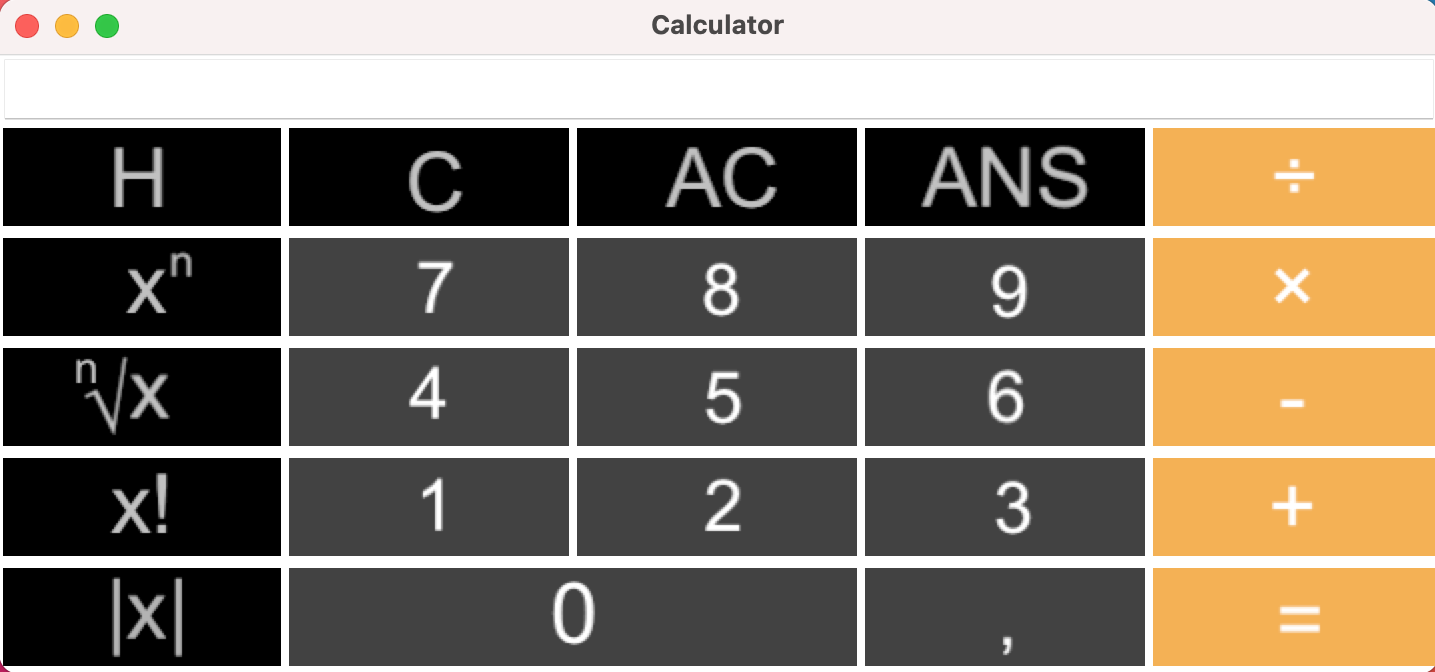
\includegraphics[scale = 0.5]{Calc_screen.png}
        \centering
        \label{fig:calc}
    \end{figure}

    \newpage

    \subsection{Math operations}
    \label{subsec:mathOperations}
    Now, the usage depends on whether you want to use binary or unary operations. \newline
    For more detailed description open refman.pdf.


    \subsubsection{Unary operations}
    First you need to enter a number then some mathematical operation. If no number is entered as the first, SYNTAX ERROR will be printed on the display.

    \subsubsection{Factorial}
    \label{subsubsec:factorial}
    \begin{figure}[hbt!]
        \caption{Factorial}
        
\includegraphics[scale = 0.2]{factorial}
        \centering
        \label{fig:fact}
    \end{figure}
    This button will calculate factorial of a number.

    \subsubsection{Absolute value}
    \label{subsubsec:absolute_value}
    \begin{figure}[hbt!]
        \caption{Absolute value}
        
\includegraphics[scale = 0.2]{abs}
        \centering
        \label{fig:abs_v}
    \end{figure}
    This button will return absolute value of a number.

    \subsubsection{Binary operations}
    First you need to enter a number, then some mathematical operation and then again press enter number (otherwise it will print SYNTAX ERROR on the display).



    \subsubsection{Plus}
    \label{subsubsec:plus}
    \begin{figure}[h]
        \caption{Plus}
        
\includegraphics[scale = 0.2]{plus}
        \centering
        \label{fig:plus}
    \end{figure}
    This button will add two numbers.

    \subsubsection{Minus}
    \label{subsubsec:minus}
    \begin{figure}[hbt!]
        \caption{Minus}
        
\includegraphics[scale = 0.2]{minus}
        \centering
        \label{fig:minus}
    \end{figure}
    This button will subtract two numbers.

    \subsubsection{Times}
    \label{subsubsec:times}
    \begin{figure}[hbt!]
        \caption{Multiply}
        
\includegraphics[scale = 0.2]{multiply}
        \centering
        \label{fig:mul}
    \end{figure}
    This button will multiply two numbers.

    \subsubsection{Divide}
    \label{subsubsec:division}
    \begin{figure}[hbt!]
        \caption{divide}
        
\includegraphics[scale = 0.2]{divide}
        \centering
        \label{fig:div}
    \end{figure}
    This button will divide two numbers.



    \subsubsection{Power}
    \label{subsubsec:power}
    \begin{figure}[hbt!]
        \caption{Power}
        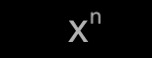
\includegraphics[scale = 0.2]{n-th_power}
        \centering
        \label{fig:pow}
    \end{figure}
    This button will calculate nth power of a number. First number is a base and second number is exponent.

    \subsubsection{Nth root}
    \label{subsubsec:nthroot}
    \begin{figure}[hbt!]
        \caption{Nth root}
        
\includegraphics[scale = 0.2]{n-th_root}
        \centering
        \label{fig:root}
    \end{figure}

    This button will calculate nth root of a number. First number is root and second number is base.
    \newpage

    \subsection{Memory oprations}
    Usage of buttons with memory operations.
    For more detailed description, open refman.pdf.
    \label{subsec:memoryoperations}

    \subsubsection{Clear Display }

    \label{subsubsec:cleardisplay}

    \begin{figure}[hbt!]
        \caption{Clear display}
        
\includegraphics[scale = 0.2]{clear_display}
        \centering
        \label{fig:ac}
    \end{figure}
    This button will clear the display. Last saved answer will remain unchanged

    \subsubsection{Clear Memory}
    \label{subsubsec:clearmemory}

    \begin{figure}[hbt!]
        \caption{Clear memory}
        
\includegraphics[scale = 0.2]{clear_memory}
        \centering
        \label{fig:c}
    \end{figure}
    This button will reset last saved answer to zero and will also clear the display

    \subsubsection{Hint}
    \label{subsubsec:hint}


    \begin{figure}[hbt!]
        \caption{Hint button}
        
\includegraphics[scale = 0.2]{hint}
        \centering
        \label{fig:h}
    \end{figure}

    This button will open up this manual.

    \subsection{Print result}
    \begin{figure}[hbt!]
        \caption{Print result}
        
\includegraphics[scale = 0.2]{plus}
        \centering
        \label{fig:print_result}
    \end{figure}

    This button has some predefined behaviour \\

    \noindent
    \textbf{1. Pressing '=' without entering first number} \\
    \indent ANS will be set on 0 and calculator will work with 0 as ANS. \\\\
    \textbf{2. Pressing '=' without previously entered math operation} \\
    \indent Last saved answer (ANS) will be printed on the display. \\\\
    \textbf{3. Pressing '=' without entering second number of binary operations} \\
    \indent SYNTAX ERROR will be printed on screen.
    \newpage

\end{document}